% --------------------------------------------------------------------------
% Шаблон презентации в стилистике Университета ИТМО
% Версия шаблона 2.1. Также шаблон доступен на сайтах:
% https://www.overleaf.com/read/rpkkfchcnbsc
% https://www.overleaf.com/latex/templates/itmo-beamer-theme/fpttrgnmqwsb
% https://github.com/AlexZabashta/ITMO-Beamer-theme
% --------------------------------------------------------------------------

% Внимание!!!
% Этот документ создан для примера использования beamer стиливика.
% Не стоит воспринимать его как урок Latex или beamer!
% Ознакомьтесь с возможностями Latex и beamer (хотя бы базовыми) отдельно.

\documentclass[aspectratio=169]{beamer}
\usepackage{presentation_style}


% Без этой команды он иногда ругается.
\hypersetup{unicode=true}

% Пакет для "русификации" Latex.
\usepackage[english,russian]{babel}

% Чтобы адекватно работало копирование текста из полученной .pdf-ки.
\usepackage{cmap}


% Это нужно, чтобы он называл рисунки без сокращения "рис.".
% Таблицы он называет без сокращения по умолчанию.
\addto\captionsrussian{\renewcommand{\figurename}{Рисунок}}

% Пакет для использования запятой в качестве десятичного разделителя.
% Следите, чтобы в формулах запятые стояли с пробелами, там где они запятые. Например $v = (x, y, z)$
\usepackage{icomma}
\usepackage{graphicx}

% Это единственный пакет для библиографии, который у меня заработал с \footcite шаблоном.
% В презентациях лучше делать её руками через \footnote!
% \usepackage[style=mla]{biblatex}
% \addbibresource{references.bib}



% По умолчанию внизу каждого слайда пишется название презентации (\inserttitle).
% Этот текст можно заменить на другой, например:
\setfootlinetext{\insertsection}


\begin{document}

\thispagestyle{empty}
\vskip 15 mm
\centerline{\footnotesize{\bf{Министерство науки высшего образования Российской Федерации}}}
\centerline{\footnotesize{{ФЕДЕРАЛЬНОЕ ГОСУДАРСТВЕННОЕ АВТОНОМНОЕ ОБРАЗОВАТЕЛЬНОЕ УЧРЕЖДЕНИЕ}}}
\centerline{\small{{ВЫСШЕГО ОБРАЗОВАНИЯ}}}
\centerline{{\bf{«НАЦИОНАЛЬНЫЙ ИССЛЕДОВАТЕЛЬСКИЙ УНИВЕРСИТЕТ ИТМО»}}}
\centerline{{\bf{(Университет ИТМО)}}}
\centerline{Факультет информационных технологий и программирования}

\vskip 30 mm
\centerline{\LARGE{ОТЧЕТ}}
\centerline{\LARGE{О НАУЧНО-ИССЛЕДОВАТЕЛЬСКОЙ РАБОТЕ}}
\vskip 2 mm
\centerline{\large{по теме:}}
\vskip 2 mm
\centerline{\large\bf{ПРОЕКТИРОВАНИЕ И РЕАЛИЗАЦИЯ РАСЧЕТНОГО МОДУЛЯ}}
\vskip 1 mm
\centerline{\large\bf{ДЛЯ СИСТЕМЫ АВТОМАТИЧЕСКОГО ФОРМИРОВАНИЯ}}
\vskip 1 mm
\centerline{\large\bf{ГЕНЕРАЛЬНЫХ ПЛАНОВ}}
\vskip 1 mm
\centerline{\large\bf{ПЛОЩАДНЫХ ОБЪЕКТОВ КАПИТАЛЬНОГО СТРОИТЕЛЬСТВА}}
\vskip 35 mm
\centerline{\large{СПИСОК ИСПОЛНИТЕЛЕЙ}}
\vskip 2 mm
\large{
\noindent
Научный руководитель, \\
Университет ИТМО, \\
факультет информационных технологий и программирования, \\
преподаватель \hskip 112 mm Пантенков С.~А.\\
\vskip 2 mm \noindent
Студент, \\
Направление подготовки 09.04.02 \\
Информационные системы и технологии, \\
Академическая группа M42051 \hskip 80 mm Степанов С.~В.\\
\vfill \hfil \break
\centerline{\large Санкт-Петербург } \centerline{ 2022 }}
\newpage


\subsection{\Large{Пользователи системы и их потребности}}
\addcontentsline{toc}{subsection}

На текущий момент невозможно полноценно реализовать систему по автоматическому
формированию генеральных планов площадных объектов в силу отсутствия методики.
Для выработки этой методики требуется провести ряд исследований в области
алгоритмов формирования генпланов.

Любые исследования для реальных промышленных задач напрямую связаны с активной консультацией с техническими
экспертами со стороны заказчика, а также грамотного оформления всех результатов проведенных исследований
и быстрой возможностью их повторения.

На время научных изысканий система будет являться исследовательским прототипом.
Она должна позволять интерактивно отображать полученные результаты и фиксировать все проведенные эксперименты.

Можно выделить три группы пользователей, которые будут взаимодействовать с системой:
\begin{enumerate}
    \item {
        \textit{Технические эксперты со стороны заказчика.} Они обладают профессиональными знаниями в сфере
        проектирования генеральных планов площадных объектов. Именно на их экспертизе и базируется итоговое
        качество получаемого решения.
    }
    \item{
        \textit{Аналитики.} Они являются связкой между техническими экспертами и исследователями.
        Именно они презентуют полученные результаты техническим экспертам и подготавливают данные в том формате,
        которым могут воспользоваться исследователи.
    }
    \item{
        \textit{Исследователи.} Основной их деятельностью является решение именно математической задачи,
        применение и обоснование методики, которая будет давать наилучший результат.
    }
\end{enumerate}

С каждой из групп пользователей было проведено интервью с целью выяснения их потребностей в работе с системой
и был составлен список этих потребностей, который представлен ниже.

\begin{enumerate}
    \item {
        \textit{Технические эксперты со стороны заказчика}
        \begin{itemize}
            \item хотят иметь интерактивный доступ к результатам исследований на различных кейсах.
        \end{itemize}
    }
    \item {
        \textit{Аналитики}
        \begin{itemize}
            \item хотят иметь возможность загрузить данные, полученные от технических экспертов,
            \item хотят оперативно видеть результаты работы команды исследователей,
            \item хотят проводить анализ результатов различных методик, полученных на разных этапах развития проекта.
        \end{itemize}
    }
    \item {
        \textit{Исследователи}
        \begin{itemize}
            \item хотят иметь удобный и простой доступ к данным, полученные от технических экспертов,
            \item хотят иметь простой способ для отправки результатов новой методики для дальнейшего анализа команде аналитиков,
            \item хотят иметь возможность оперативно добавлять новые методики в действующий функционал системы.
        \end{itemize}
    }
\end{enumerate}

На основе потребностей пользователей можно составить несколько сценариев использования системы.
Для каждой группы пользователей эти сценарии будут несколько разными.
Ниже представлена диаграмма вариантов использования(см. рис\ \ref{pic:analysis__usecases-usecase}).

\begin{figure}[H]
	\hspace*{-2.5 cm}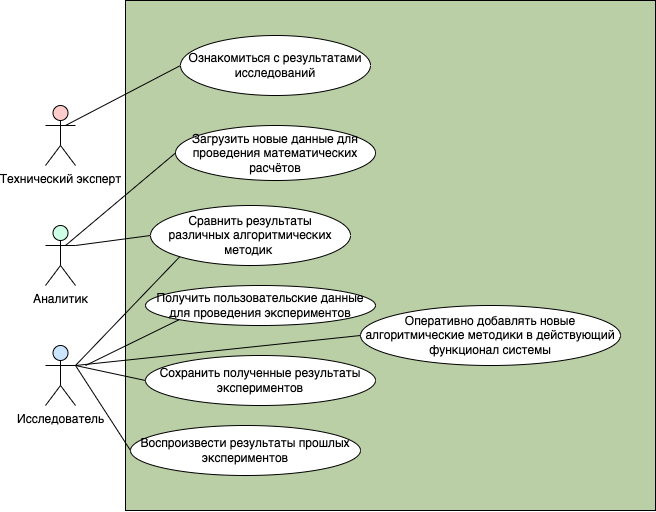
\includegraphics[width=0.6\textwidth, left]{analysis/pictures/usecases/usecase}
	\caption{Диаграмма вариантов использования}
	\label{pic:analysis__usecases-usecase}
\end{figure}
\vskip 5 mm



\section{Second Section}

\begin{frame}
\frametitle{Blocks of Highlighted Text}
\begin{block}{Regular Block}
Lorem ipsum dolor sit amet, consectetur adipiscing elit. Integer lectus nisl, ultricies in feugiat rutrum, porttitor sit amet augue. Aliquam ut tortor mauris. Sed volutpat ante purus, quis accumsan dolor.
\end{block}

\begin{exampleblock}{Example Block}
Pellentesque sed tellus purus. Class aptent taciti sociosqu ad litora torquent per conubia nostra, per inceptos himenaeos. Vestibulum quis magna at risus dictum tempor eu vitae velit.
\end{exampleblock}

\begin{alertblock}{Alert Block}
Suspendisse tincidunt sagittis gravida. Curabitur condimentum, enim sed venenatis rutrum, ipsum neque consectetur orci, sed blandit justo nisi ac lacus.
\end{alertblock}
\end{frame}


\begin{frame}
\frametitle{Colors}

You can use main official predefined colors
\textcolor{ITMOblue}{ITMOblue} and \textcolor{ITMOred}{ITMOred}, and also
 \textcolor{ITMOorange}{ITMOorange}, \textcolor{ITMOsky}{ITMOsky}, \textcolor{ITMOpistachio}{ITMOpistachio}, \textcolor{ITMOaqua}{ITMOaqua}, \textcolor{ITMOice}{ITMOice}, \textcolor{ITMOgold}{ITMOgold}, \textcolor{ITMOyellow}{ITMOyellow}, \textcolor{ITMOtomato}{ITMOtomato}, \textcolor{ITMOgreen}{ITMOgreen}.

\end{frame}



\subsection{Using columns}


\begin{frame}
\frametitle{Multiple Columns}
\begin{columns}[c]

\column{.45\textwidth}{
    \begin{enumerate}
        \item First item
        \item Second item
        \item Third item
    \end{enumerate}
}

\column{.45\textwidth}{
    \begin{itemize}
        \item Some item
        \item Another item
        \item Also item
    \end{itemize}
}

\end{columns}
\end{frame}



\section{Other LaTex stuff}

\subsection{Tables}


\begin{frame}
\frametitle{Table}

% Лучше не использовать table в презентациях, только tabular. А описание таблиц делать руками.

\begin{table}
\caption{Multiplication table of complex numbers}
\begin{tabular}{r | r r r r r}
$a \times b$ & $0$ &  $1$ &  $i$ & $-1$ & $-i$ \\ \hline
         $0$ & $0$ &  $0$ &  $0$ &  $0$ &  $0$ \\
         $1$ & $0$ &  $1$ &  $i$ & $-1$ & $-i$ \\
         $i$ & $0$ &  $i$ & $-1$ & $-i$ &  $1$ \\
        $-1$ & $0$ & $-1$ & $-i$ &  $1$ &  $i$ \\
        $-i$ & $0$ & $-i$ &  $1$ &  $i$ & $-1$ \\
\end{tabular}
\end{table}
\end{frame}


\subsection{Theorems and Equations}


\begin{frame}
\frametitle{Theorem}
\begin{theorem}[Fermat's Last Theorem]
\begin{equation}
    \forall n, x, y, z \in \mathbb{N}: \mathbf{n > 2} \Rightarrow x^n + y^n \neq z^n
\end{equation}
\end{theorem}
I have discovered a truly remarkable proof of this theorem which this frame is too small to contain.
\end{frame}


\subsection{Figures}


\begin{frame}
\frametitle{Figure example}
\begin{figure}
    \includegraphics[scale=.3]{fig/parabola.png}
    \caption{Parabola with focus and directrix}
\end{figure}
\end{frame}

\begin{frame}[plain]
    \itmopolygons{
        \vfill
        \Huge{Спасибо за внимание!}
        \vfill
        
\includegraphics[scale=.5]{itmo/slogan}
    }
\end{frame}
\end{document}
